\chapter{Parallel Programming Models}
In this section different parallel programming models are discussed, together with their advantages and disadvantages.

\begin{figure}
	\centering
	\subfloat[Shared Memory] {
		\input{Tikz/SharedMemory}
		\label{fig:shared_memory}
	}
	$\hspace{36pt}$
	\subfloat[Distributed Memory] {
		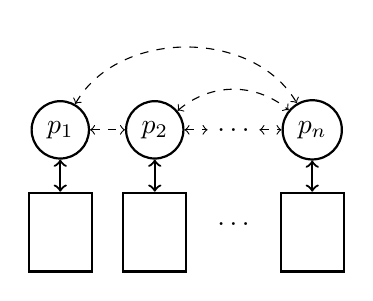
\begin{tikzpicture}
\node[circle, thick, draw] (v1) at (-0.2,0.8) {$p_1$};
\node[circle, thick, draw] (v3) at (1,0.8) {$p_2$};
\node (v7) at (2,0.8) {$\dots$};
\node at (2,-0.4) {$\dots$};
\node[circle, thick, draw] (v5) at (3,0.8) {$p_n$};

\node (v2) at (-0.2,-0.11) {};
\node (v4) at (1,-0.11) {};
\node (v6) at (3,-0.11) {};

\draw[thick] (-0.6,0) rectangle (0.2,-1);
\draw[thick]  (0.6,0) rectangle (1.4,-1);
\draw[thick]  (2.6,0) rectangle (3.4,-1);

\draw[<->, thick]  (v1) edge (v2);
\draw[<->, thick]  (v3) edge (v4);
\draw[<->, thick]  (v5) edge (v6);

\draw[<->, dashed]  (v1) edge (v3);
\draw[<->, dashed]  (v3) edge (v7);
\draw[<->, dashed]  (v7) edge (v5);
\draw[<->, dashed]  (v3) edge [bend left=40 ] (v5) ;
\draw[<->, dashed]  (v1) edge [bend left=60 ] (v5);

\end{tikzpicture}
		\label{fig:distributed_memory}
	}

	\caption{Here $n$ processes $p_1, \dots, p_n$ are displayed in a \emph{Shared Memory} and a \emph{Distributed Memory} setting. Dashed edges represent communication links between processes.}
	\label{fig:shared_distributed_memory}
\end{figure}

\section{Shared Memory Architecture}
In a \emph{Shared Memory Architecture (SMA)}, all processes work in a shared address space, like shown in Figure \ref{fig:shared_memory}. Note that interprocess communication is done implicitly, since every process can access the entire address space.

Since the entire available memory can be accessed via a shared address space, the shared memory model simplifies programming. Algorithms with challenging data dependencies can be modelled elegantly in shared memory. A disadvantage is that data locality is not taken into account, because processes are not aware where data resides. This could bring performance penalties.

\subsection{NUMA}
An example of a shared memory architecture is \emph{Non-Uniform Memory Access (NUMA)}, a model used in computer systems with multiple CPUs. In NUMA every CPU has a local memory and and every CPU can access memory local to other CPUs via a shared address space. Some parts of the address space are on different buses than others, so different parts of the address space may differ in performance. This makes memory accesses non-uniformly.

NUMA is contrasted with \emph{Uniform Memory Access (UMA)}, in which all CPUs share the same physical memory uniformly.

\subsection{SMP}
Another example of shared memory architectures is the \emph{Symmetric Multiprocessing (SMP)} architecture. In SMP all CPUs access memory via the same shared memory bus. Memory-intensive algorithms generally perform better under the NUMA architecture, since the single memory bus in SMP can easily become a performance bottleneck.

\section{Distributed Memory Architecture}
Figure \ref{fig:distributed_memory} shows a \emph{Distributed Memory Architecture (DMA)}. In DMA every process can only access its private memory. When a process needs to access memory that is private to another process, it needs to do so via message passing. This is represented in Figure \ref{fig:distributed_memory} by the dashed edges between processes. 

DMA is widely used to create distributed programs, i.e. programs that run on a cluster of computing machines. Every participating machines has a CPU and main memory, which fits perfectly in the distributed memory model. Machines can send messages to each other via the network. DMA can also be used on a single machine if the available memory is large enough. A popular interface for message passing is the \emph{Message Passing Interface (MPI)}. Applications using the distributed memory model generally use the SPMD programming style.

An advantage of DMA is that data locality is fully exploited, since processes only access local memory. Also programs created with the distributed memory model can easily be distributed across a cluster of machines. Memory management on the other hand is a lot harder, because the available memory is distributed.

\begin{figure}
	\centering
	\subfloat[PGAS] {
		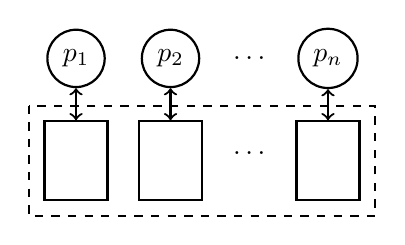
\begin{tikzpicture}
\node[circle, thick, draw] (v1) at (-0.2,0.8) {$p_1$};
\node[circle, thick, draw] (v3) at (1,0.8) {$p_2$};
\node (v7) at (2,0.8) {$\dots$};
\node at (2,-0.4) {$\dots$};
\node[circle, thick, draw] (v5) at (3,0.8) {$p_n$};

\node (v2) at (-0.2,-0.11) {};
\node (v4) at (1,-0.11) {};
\node (v6) at (3,-0.11) {};

\draw[thick] (-0.6,0) rectangle (0.2,-1);
\draw[thick]  (0.6,0) rectangle (1.4,-1);
\draw[thick]  (2.6,0) rectangle (3.4,-1);

\draw[<->, thick]  (v1) edge (v2);
\draw[<->, thick]  (v3) edge (v4);
\draw[<->, thick]  (v5) edge (v6);

\draw[thick, dashed]  (-0.8,0.2) rectangle (3.6,-1.2);
\end{tikzpicture}
		\label{fig:pgas}
	}
	$\hspace{36pt}$
	\subfloat[Hybrid PGAS+MPI] {
		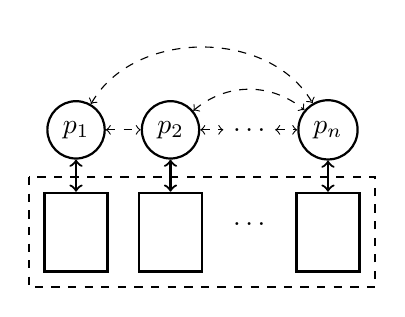
\begin{tikzpicture}
\node[circle, thick, draw] (v1) at (-0.2,0.8) {$p_1$};
\node[circle, thick, draw] (v3) at (1,0.8) {$p_2$};
\node (v7) at (2,0.8) {$\dots$};
\node at (2,-0.4) {$\dots$};
\node[circle, thick, draw] (v5) at (3,0.8) {$p_n$};

\node (v2) at (-0.2,-0.11) {};
\node (v4) at (1,-0.11) {};
\node (v6) at (3,-0.11) {};

\draw[thick] (-0.6,0) rectangle (0.2,-1);
\draw[thick]  (0.6,0) rectangle (1.4,-1);
\draw[thick]  (2.6,0) rectangle (3.4,-1);

\draw[<->, thick]  (v1) edge (v2);
\draw[<->, thick]  (v3) edge (v4);
\draw[<->, thick]  (v5) edge (v6);

\draw[thick, dashed]  (-0.8,0.2) rectangle (3.6,-1.2);

\draw[<->, dashed]  (v1) edge (v3);
\draw[<->, dashed]  (v3) edge (v7);
\draw[<->, dashed]  (v7) edge (v5);
\draw[<->, dashed]  (v3) edge [bend left=40 ] (v5) ;
\draw[<->, dashed]  (v1) edge [bend left=60 ] (v5);
\end{tikzpicture}
		\label{fig:pgas_hybrid}
	}
	\caption{Here $n$ processes $p_1, \dots, p_n$ are displayed in an \emph{PGAS} setting. Every process can access the entire combined memory, of which a small portion is local. The global address spaces are represented by dashed rectangles and the local address spaces by solid rectangles. }
	\label{fig:pgas_hybrid_pgas}
\end{figure}

\section{Partitioned Global Address Space}
The shared and distributed memory models can be combined into a \emph{distrbited shared memory} model. This is shown in Figure \ref{fig:pgas}. Every process has a local memory and all local memories are combined into a single global address space. This model is called \emph{Partitioned Global Address Space (PGAS)}, since the global address space is partitioned by the local memories of the participating processes. This makes PGAS a NUMA architecture.

PGAS combines most of the advantages of both the shared and distributed (SPMD) memory models. Data locality is exploited because every process knows its local memory. PGAS can be used both on a single computer and on a cluster of computers, because of its distributed structure. This simplifies programming systems to scale both parallel and distributed. 

\subsection{Asynchronous Partitioned Global Address Space}
A variant to PGAS is the \emph{Asynchronous Partitioned Global Address Space (APGAS)} model \cite{APGAS}. In APGAS the PGAS model is extended with tasks and task pools. Every node can asynchronously create and execute tasks both locally and remotely. Dynamic load-balancing is automatically applied over tasks. The PGAS model implicitly assumes all processes to run on similar hardware. APGAS has a richer execution framework due to its task-based structure and works well on non-uniform clusters.

\subsection{PGAS and MPI}
A \emph{Hybrid PGAS+MPI} parallel programming model can be used by combining PGAS with the distributed memory model. This is shown in Figure \ref{fig:pgas_hybrid}. In this model processes are able to perform message passing in addition to PGAS. The hybrid model can be used to implement software that does not entirely fit into the PGAS model. Also legacy code written for MPI can benefit from this model.

\subsection{PGAS and RDMA}
If PGAS is used in a distributed setting, it can be combined with RDMA. Every process creates an address space using virtual memory as an abstraction to the entire available memory. Local memory operations can simply be performed and remote operations are translated into one-sided RDMA operations. This makes the combination of RDMA and PGAS a high-performance parallel and distributed platform. 

\section{Parallel Programming Libraries}
This section introduces several parallel programming libraries that can be used in the research project.

\subsection{Message Passing Interface}
The \emph{Message Passing Interface (MPI)} is a popular interface for process communication written in C. With MPI processes can communicate by exchanging messages. MPI is used to create scalable parallel programs, as well as distributed programs.

MPI-3 supports one-sided communication and \emph{Remote Memory Access (RMA)} \cite{conf/sc/GerstenbergerBH13}, so MPI-3 is not longer limited to message passing alone. Many implementations of MPI-3 use RDMA when available to implement the one-sided operations and RMA. MPI also supports the shared memory model \cite{mpi-shared-mem-win}. 

\subsubsection{RMA and RDMA}
The difference between RMA and RDMA is that RDMA requires specialized hardware to directly access remote memory. Remote memory access can still be performed when RMDA-enabled hardware is not available by involving the OS kernel. MPI thus supports the use of remote memory calls without the need of specialized hardware by dropping the requirement of directly accessing remote memory. Many implementations of MPI however do use RDMA when the hardware enables it.

\subsubsection{MVAPICH2}
\emph{MVAPICH2} \cite{mvapich2} is an efficient implementation of MPI-3 for Infiniband hardware. It is efficient in the sense that hardware optimizations are used where possible. MVAPICH comes with a number of variants, one of which is \emph{MVAPICH2-X}, which supports PGAS and the hybrid PGAS/MPI model on Infiniband hardware. This implementation can be used with the PGAS models UPC and OpenSHMEM \cite{implementing_openshmem}. 

\subsubsection{PGAS and GPUs}
Another variant is \emph{MVAPICH2-GDR} \cite{Wang:2011:MOG:1997883.1997893}, which makes use of the GPUDirect RDMA technology \cite{gpudirect}. With MVAPICH2-GDR algorithms can be designed to operate on GPU clusters. It would be possible to design heterogeneous algorithms by combining MVAPICH2-X and MVAPICH2-GDR, but this is future work.

\subsection{PGAS Languages}
A number of PGAS languages exist, including Unified Parallel C (UPC), Co-array Fortran (CAF), Titanium, X10, Chapel, and OpenSHMEM. The languages UPC, CAS, and Titanium are extensions to C, Fortran, and Java, respectively. 

\subsubsection{APGAS implementations}
Chapel and X10 are both implementations of the APGAS model \cite{Chamberlain:2007:PPC:1286120.1286123, Charles:2005:XOA:1103845.1094852}. Both are actual programming languages influenced by C++ and Java. These languages provide direct support for PGAS, task management and the dynamic load balancing of tasks. A disadvantage is that both langauges structurally differ from C, so the existing BDD operations written in C all have to be rewritten if X10 or Chapel is used. Also interoperability with LTSmin could be problematic, so these two languages are not used further in this research project.

\subsubsection{OpenSHMEM}
OpenSHMEM (Open Shared Memory) is a specification for a standard API for parallel programming in PGAS \cite{openshmem}. Several implementations of OpenSHMEM exist, including an implementation for MVAPICH2-X. The performance of MVAPICH2-X in combination with OpenSHMEM is evaluated in \cite{openshmem_perf_evaluation} and compared to other OpenSHMEM libraries. The experiments were performed on the TACC Stampede cluster \cite{stampede_cluster}. The researchers concluded that this combination delivered best performance and scalability. Especially the atomic and collective operations performed significantly better due to the efficient use of Infiniband hardware. The atomic operations include \texttt{compare-and-swap} and \texttt{fetch-and-add} and the collective operations include \texttt{broadcast}, \texttt{reduce}, \texttt{collect}, and \texttt{barrier}. 

Note that MVAPICH2-X can also be used in combination with UPC. Although this combination is not benchmarked in \cite{openshmem_perf_evaluation}, the benchmarks presented on the MVAPICH2 website point out that UPC performs slightly better.